\section{Ejemplos de aplicación}

\subsection{Movimiento por fuerza boyante en un circuito cerrado}

\begin{frame}
{Ejemplos de aplicación}
{Fluidodinámica en una fuente fría de neutrones}

\begin{figure}
\centering{}
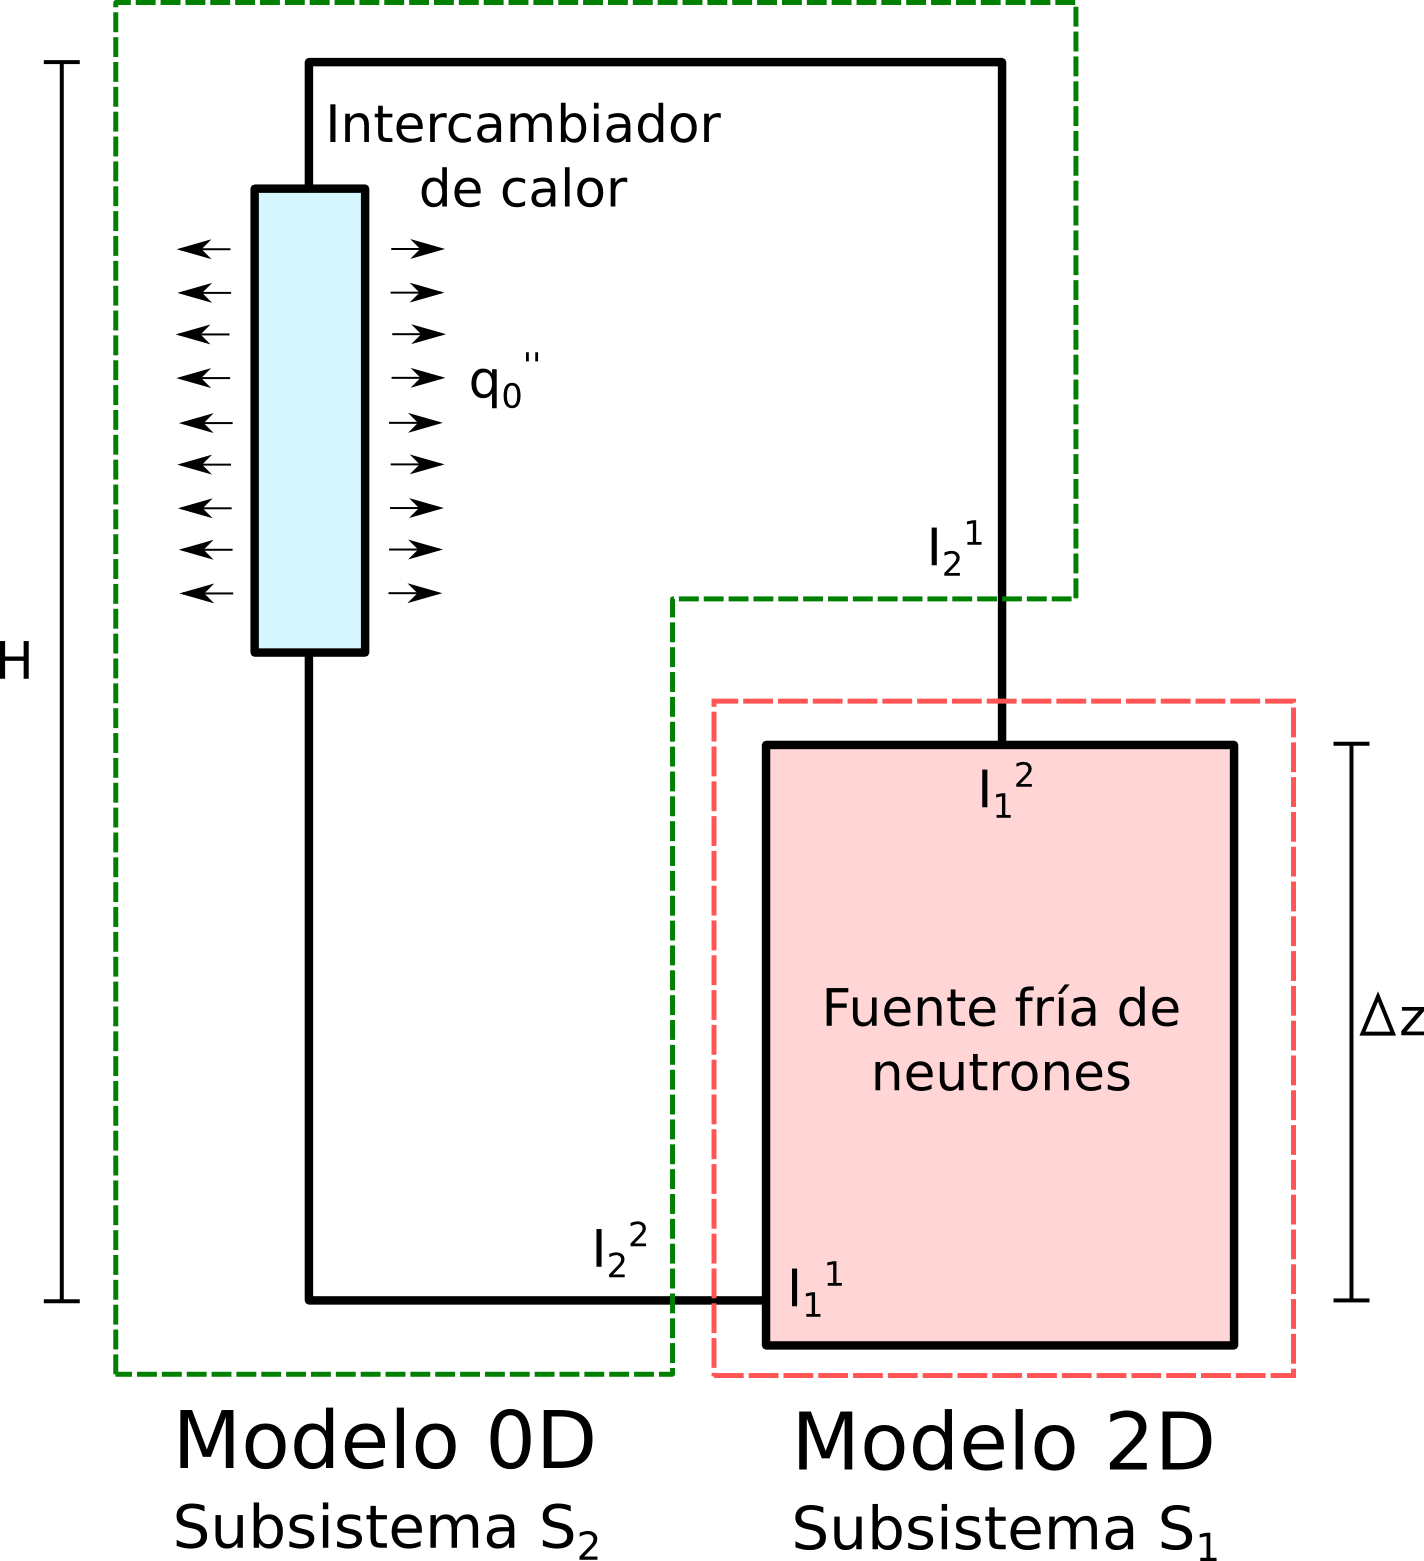
\includegraphics[scale=0.27]{fuente-fria.png}
\end{figure}

\end{frame}

\begin{frame}
{Ejemplos de aplicación}
{Fluidodinámica en una fuente fría de neutrones}

Sistema $S_1$:

\visible<2->{
Parámetros utilizados: $\rho_0=163$ $Kg/m^3$ a la temperatura de referencia $T_{ref}$,
$\mu=2.8\cdot 10^{-5}$ $Kg/ms$, $c_p=6333.6$ $J/KgK$, 
$k=0.136$ $W/mK$ y $\beta=1.32\cdot10^{-2}K^{-1}$.
Las áreas de las interfaces de acople son $A_2^1=A_2^2=0.03$ $m^2$.
}

\visible <3>{
\begin{equation*}
\left\{ \begin{array}{lr}
\displaystyle \frac {\partial \bar{u}}{\partial t} + ( \bar{u} \cdot \nabla) \bar{u} = - \frac {\nabla p}{\rho_0}
+ \left( 1- \beta (T-T_{ref}) \right)\bar{g} + \\ [0.24cm]
+ \nabla \cdot \left[ \left( \nu\right) \left( \nabla \bar{u} + \nabla \bar{u}^T \right) \right] \\ [0.2cm]
\nabla \cdot \bar{u} = 0 \\ [0.2cm]
\displaystyle \frac {\partial T}{\partial t} + ( \bar{u} \cdot \nabla) T = \frac {k}{\rho_0 c_p} \Delta T + \frac{f_0}{\rho_0 c_p}
\label{eq-cavidad}
\end{array}
\right.
\end{equation*}
donde $\bar{u}$ es el campo de velocidades dentro de la cavidad,
$p$ el campo de presiones y
$T$ el campo de temperaturas.
}

\end{frame}

\begin{frame}
{Ejemplos de aplicación}
{Fluidodinámica en una fuente fría de neutrones}

Sistema $S_2$:

\visible<2->{
Parámetros extra utilizados:
longitud total de cañerías $L=15$ $m$, 
sumatoria de coeficientes de pérdida de carga concentrada $\sum K_i=1.72$, 
rugosidad de cañerías $\epsilon=0.5\cdot 10^{-4}$ $m$.
}

\visible <3>{
\begin{equation*}
\left\{ \begin{array}{l}
Q_2^{2} = Q_2^{1} \\ [0.2cm]
p_2^2 = p_2^1 + \rho_0 g \left ( \Delta z + \beta (T_2^1 - T_{ref}) (H-\Delta z) \right ) - \\ [0.2cm]
- \rho_0 \frac{1}{2} \left( \frac{Q_1^1}{A_2^1} \right)^2  \left( \frac {f_D L} {D} + \sum_i K_i \right)  \\ [0.2cm]
T_2^2 = 0
%T_2^2 =& T_2^1 + 2 \frac {q_0" L}{\frac{D}{2} \frac{Q_1^1}{A_2^1}\rho c_p}
\label{eq-intercambiador}
\end{array}
\right.
\end{equation*}
donde $Q_2^i$ es el caudal en la interfaz $i$,
$p_2^i$ es la presión del subsistema promediada en esta interfaz,
$T_2^i$ es la temperatura promediada en esta interfaz,
$g$ es la aceleración generada por el campo gravitatorio,
$f_D$ es el factor de $Darcy$ de pérdida de carga distribuida,
y $D$ es el diámetro de la tubería.
}
\end{frame}

\begin{frame}
{Ejemplos de aplicación}
{Fluidodinámica en una fuente fría de neutrones}

Estrategia de resolución:

\begin{itemize}
\item Ecuaciones de continuidad
\begin{equation*}
\left\{ \begin{array}{l}
Q_1^1= Q_2^2 \\
Q_1^2= Q_2^1 \\
p_1^1= p_2^2 \\
p_1^2= p_2^1 \\
T_2^1= T_2^2 \\
T_2^2= T_2^1 \\
q"_2^1= - q"_2^2 \\
q"_2^2= - q"_2^1
\end{array}
\right.
\end{equation*}
\end{itemize}

\end{frame}

\begin{frame}
{Ejemplos de aplicación}
{Fluidodinámica en una fuente fría de neutrones}

\begin{itemize}
\item Selección de condiciones de borde
  \begin{itemize}
  \item en la interfaz inferior de la cavidad 2-D:
      \begin{itemize}
      \item condiciones de tipo \textit{Dirichlet} para el par presión-caudal
      \item condiciones de tipo \textit{Dirichlet} para el par temperatura-flujo de calor
      \end{itemize}
  \item en la interfaz superior de la cavidad 2-D:
      \begin{itemize}
      \item condiciones de tipo \textit{Neumann} para el par presión-caudal
      \item condiciones de tipo \textit{Neumann} para el par temperatura-flujo de calor
      \end{itemize}
  \visible<2>{\item en la interfaz inferior de la red 0-D:
      \begin{itemize}
      \item condiciones de tipo \textit{Neumann} para el par presión-caudal
      \item condiciones de tipo \textit{Neumann} para el par temperatura-flujo de calor
      \end{itemize}
  \item en la interfaz superior de la red 0-D:
      \begin{itemize}
      \item condiciones de tipo \textit{Neumann} para el par presión-caudal
      \item condiciones de tipo \textit{Dirichlet} para el par temperatura-flujo de calor
      \end{itemize}}
  \end{itemize} 

\end{itemize}

\end{frame}



\begin{frame}
{Ejemplos de aplicación}
{Fluidodinámica en una fuente fría de neutrones}

\begin{itemize}
\item Ecuaciones de residuos en subsistema 1:

\begin{equation*}
\left\{ \begin{array}{l}
(R_{p,Q})_{1}^{1}  = p_1^{1, guess} - p_1^{1, calc}(Q_1^{1, guess}, T_1^{1, guess}, p_1^{2, guess}, q_1''^{2, guess}) \\
(R_{T,q"})_{1}^{1} = q_{1}''^{1, guess} - q_{1}''^{1, calc}(Q_1^{1, guess}, T_1^{1, guess}, p_1^{2, guess}, q_1''^{2, guess}) \\
(R_{p,Q})_{1}^{2}  = Q_1^{2, guess} - Q_1^{2, calc}(Q_1^{1, guess}, T_1^{1, guess}, p_1^{2, guess}, q_1''^{2, guess}) \\
(R_{T,q"})_{1}^{2} = T_1^{2, guess} - T_1^{2, calc}(Q_1^{1, guess}, T_1^{1, guess}, p_1^{2, guess}, q_1''^{2, guess})
\end{array}
\right.
\label{residuos-1}
\end{equation*}

\item <2-> Ecuaciones de residuos en subsistema 2:

\begin{equation*}
\left\{ \begin{array}{l}
(R_{p,Q})_{2}^{1}  = Q_2^{1, guess} - Q_2^{1, calc}(p_2^{1, guess}, T_2^{1, guess}, p_2^{2, guess}, q_2''^{2, guess}) \\
(R_{T,q"})_{2}^{1} = q_{2}''^{1, guess} - q_{2}''^{1, calc}(p_2^{1, guess}, T_2^{1, guess}, p_2^{2, guess}, q_2''^{2, guess}) \\
(R_{p,Q})_{2}^{2}  = Q_2^{2, guess} - Q_2^{2, calc}(p_2^{1, guess}, T_2^{1, guess}, p_2^{2, guess}, q_2''^{2, guess})  \\
(R_{T,q"})_{2}^{2} = T_2^{2, guess} - T_2^{2, calc}(p_2^{1, guess}, T_2^{1, guess}, p_2^{2, guess}, q_2''^{2, guess}) 
\end{array}
\right.
\label{residuos-2}
\end{equation*}

\end{itemize}

\end{frame}

\begin{frame}
{Ejemplos de aplicación}
{Fluidodinámica en una fuente fría de neutrones}

\begin{itemize}
\item Ecuaciones de residuos en subsistema 1: (fijo $p_1^2=p_{ref}=0$)

\begin{equation*}
\left\{ \begin{array}{l}
(R_{p,Q})_{1}^{1}  = p_1^{1, guess} - p_1^{1, calc}(Q_1^{1, guess}, T_1^{1, guess}, p_1^{2, guess}, q_1''^{2, guess}) \\
(R_{T,q"})_{1}^{1} = q_{1}''^{1, guess} - q_{1}''^{1, calc}(Q_1^{1, guess}, T_1^{1, guess}, p_1^{2, guess}, q_1''^{2, guess}) \\
$\sout{$(R_{p,Q})_{1}^{2} = Q_1^{2, guess} - Q_1^{2, calc}(Q_1^{1, guess}, T_1^{1, guess}, p_1^{2, guess}, q_1''^{2, guess})$}$ \\
(R_{T,q"})_{1}^{2} = T_1^{2, guess} - T_1^{2, calc}(Q_1^{1, guess}, T_1^{1, guess}, p_1^{2, guess}, q_1''^{2, guess})
\end{array}
\right.
\label{residuos-1}
\end{equation*}

\item Ecuaciones de residuos en subsistema 2: (fijo $p_2^1=p_{ref}=0$)

\begin{equation*}
\left\{ \begin{array}{l}
$\sout{$(R_{p,Q})_{2}^{1}  = Q_2^{1, guess} - Q_2^{1, calc}(p_2^{1, guess}, T_2^{1, guess}, p_2^{2, guess}, q_2''^{2, guess})$}$  \\
(R_{T,q"})_{2}^{1} = q_{2}''^{1, guess} - q_{2}''^{1, calc}(p_2^{1, guess}, T_2^{1, guess}, p_2^{2, guess}, q_2''^{2, guess}) \\
(R_{p,Q})_{2}^{2}  = Q_2^{2, guess} - Q_2^{2, calc}(p_2^{1, guess}, T_2^{1, guess}, p_2^{2, guess}, q_2''^{2, guess})  \\
(R_{T,q"})_{2}^{2} = T_2^{2, guess} - T_2^{2, calc}(p_2^{1, guess}, T_2^{1, guess}, p_2^{2, guess}, q_2''^{2, guess}) 
\end{array}
\right.
\label{residuos-2}
\end{equation*}

\end{itemize}

\end{frame}




\begin{frame}
{Ejemplos de aplicación}
{Fluidodinámica en una fuente fría de neutrones}
Distintos comportamientos según el $Ri$ obtenido:
\begin{itemize}
\item $Ri=0.8$:
\end {itemize}

\begin{center}
\movie[width=0.7\textwidth,showcontrols=true]
{% placeholder = text or image
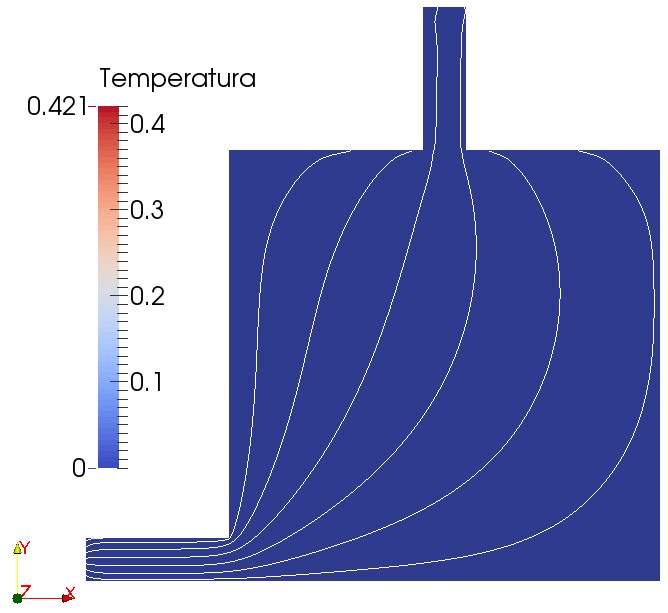
\includegraphics[width=0.5\textwidth]{ri-portada.png}
}%
{figs/ri08.ogv} % video filename
\end{center}

\end{frame}


\begin{frame}
{Ejemplos de aplicación}
{Fluidodinámica en una fuente fría de neutrones}
Distintos comportamientos según el $Ri$ obtenido:
\begin{itemize}
\item $Ri=84$:
\end {itemize}

\begin{center}
\movie[width=0.7\textwidth,showcontrols=true]
{% placeholder = text or image
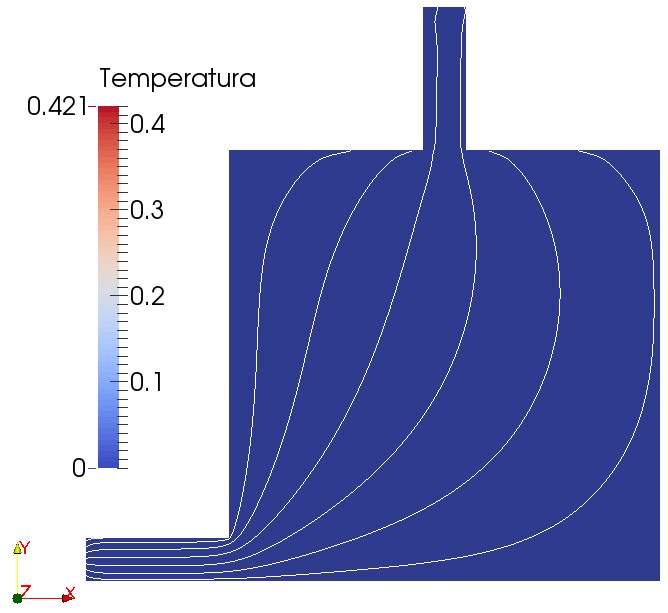
\includegraphics[width=0.5\textwidth]{ri-portada.png}
}%
{figs/ri84.ogv} % video filename
\end{center}

\end{frame}




\begin{frame}
{Ejemplos de aplicación}
{Fluidodinámica en una fuente fría de neutrones}

A mayor altura $H$ del intercambiador de calor, mayor caudal obtenido:

\begin{table}[h!]
  \centering
  \begin{tabular}{ c c c c c c c } 
      \hline
      \multicolumn{1}{c}{$f_0$ $[W/m^3]$} & \multicolumn{1}{c}{$H / \Delta z$} & \multicolumn{1}{c}{$Ri$} & \multicolumn{1}{c}{$\Delta T$ $[K]$} & \multicolumn{1}{c}{$Q$$[m^3/s]$}& \multicolumn{1}{c}{$\Delta p$ $[Pa]$} \\ \hline
      \multirow{3}{*}{$2\cdot10^4$} & $1$ & 3.4 & 0.7 & $3.2 \cdot 10^{-3}$ & 613 \\
                         & $5$ & 1 & 0.5 & $4.2 \cdot 10^{-3}$ & 614 \\
                         & $10$ & 0.5 & 0.3 & $4.5 \cdot 10^{-3}$ & 617 \\ \hline
      \multirow{3}{*}{$2\cdot10^5$} & $1$ & 6.5 & 3.6 & $4.4 \cdot 10^{-3}$ & 595 \\
                         & $5$ & 1.7 & 2.8 & $7.6 \cdot 10^{-3}$ & 605 \\
                         & $10$ & 0.9 & 2.2 & $9.0 \cdot 10^{-3}$ & 620 \\ \hline
      \multirow{3}{*}{$2\cdot10^6$} & $1$ & 10.6 & 24 & $8.9 \cdot 10^{-3}$ & 465 \\
                         & $5$ & 2.2 & 18 & $1.7 \cdot 10^{-2}$ & 580 \\
                         & $10$ & 0.9 & 11.6 & $2.1 \cdot 10^{-2}$ & 700 \\ \hline
   \end{tabular}   
   \caption[Principales resultados del cálculo para el análisis de la fuente fría variando la magnitud de la fuente interna y la altura del sistema de enfriamiento]
   {Principales resultados del cálculo para el análisis de la fuente fría variando la magnitud de la fuente interna y la altura del sistema de enfriamiento.}
   \label{tab-deuterio}
\end{table}

\end{frame}


\begin{frame}
{Ejemplos de aplicación}
{Fluidodinámica en una fuente fría de neutrones}

Análisis de métodos de resolución del sistema de ecuaciones de residuos:

\begin{figure}
\centering{}
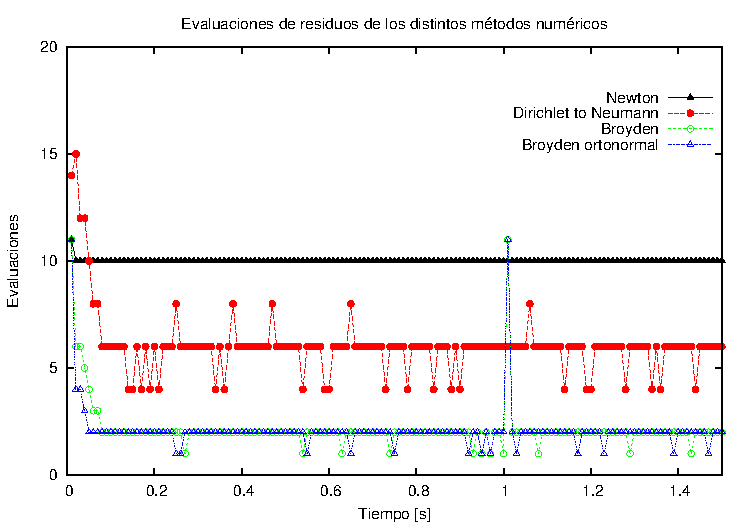
\includegraphics[scale=0.7]{evaluaciones-ff.pdf}
\end{figure}

\end{frame}












\subsection{Análisis del segundo sistema de parada de un reactor de investigación}

\begin{frame}
{Ejemplos de aplicación}
{Análisis del segundo sistema de parada de un reactor de investigación}

Esquema del Segundo Sistema de Parada (SSP) del RA-10:

\begin{figure}
\centering{}
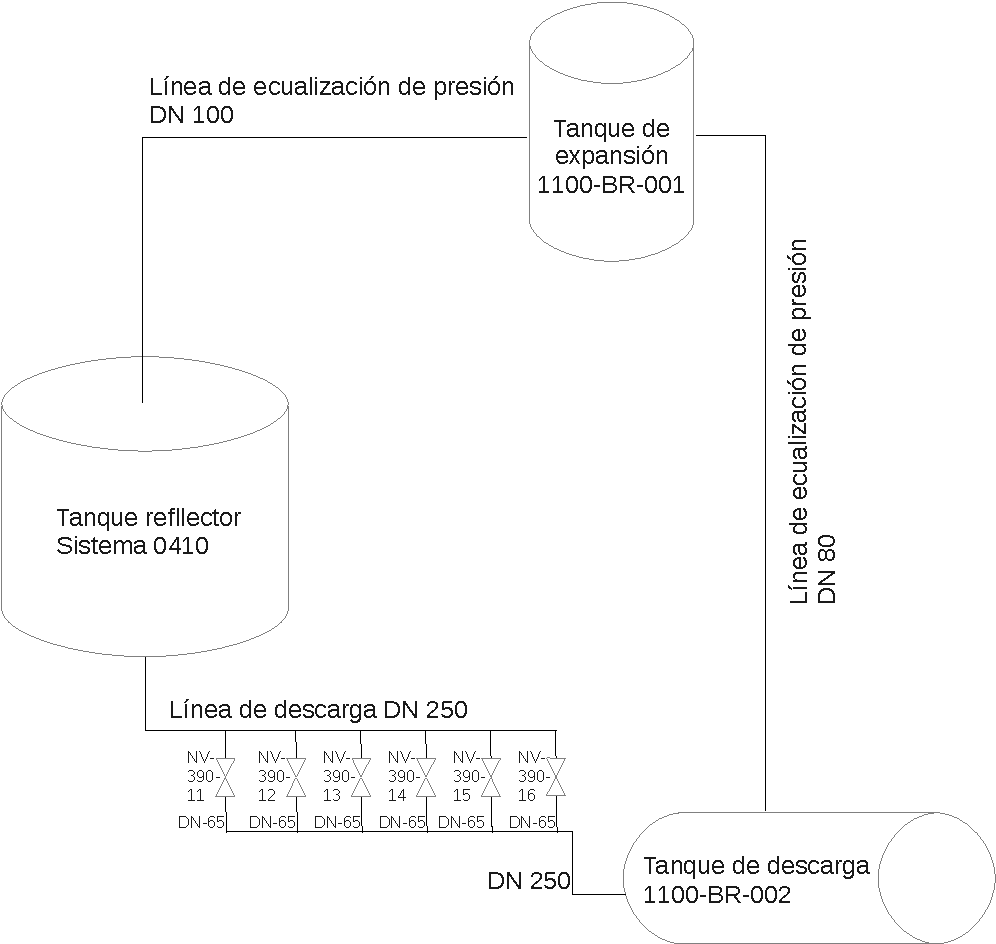
\includegraphics[scale=0.42]{SSP.pdf}
\end{figure}

\end{frame}

\begin{frame}
{Ejemplos de aplicación}
{Análisis del segundo sistema de parada de un reactor de investigación}

Subdominios de análisis:

\begin{itemize}
\item <2-> Subsistema del tanque del reflector,
\item <3-> Subsistema de la red hidráulica de descarga,
\item <4-> Subsistema de la red hidráulica de ecualización de presiones.
\end{itemize}

\end{frame}

\begin{frame}
{Ejemplos de aplicación}
{Análisis del segundo sistema de parada de un reactor de investigación}

Subdominios de análisis:

\begin{itemize}
\item Subsistema del tanque del reflector (0-D),
\item Subsistema de la red hidráulica de descarga (3-D),
\item \sout{Subsistema de la red hidráulica de ecualización de presiones}.
\end{itemize}

\end{frame}

% \tiny
% \scriptsize
% \footnotesize
% \small	
% \normalsize
% \large
% \Large
% \LARGE
% \huge
% \Huge

\footnotesize
\begin{frame}
{Ejemplos de aplicación}
{Análisis del segundo sistema de parada de un reactor de investigación}

Subsistema 0-D:

\begin{equation*}
\ddot{h} h + \frac{\dot{h}^2}{2}\left( 1- \left(\frac{A_T}{A_D} \right)^2 \right) + g \Delta h_{red} + \ddot{h}  l_D = 
\frac{p_{atm}-p_1^1}{\rho} + \Delta \hat{u}
\label{eq-tanque}
\end{equation*}
donde $p_1^1$ es la presión en la interfaz de acople,
$A_T$ es la área transversal del tanque del reflector, 
$A_D$ es la sección transversal de la línea de descarga,
$\Delta h_{red}$ es la altura total de la columna de líquido en el subsistema,
$l_D$ es la longitud total de cañerías en el subsistema,
$p_{atm}$ es la presión sobre la superficie libre,
y $\rho$ es la densidad del agua.
$\Delta \hat{u}$ representa la pérdida de carga por unidad de masa y puede modelarse como:

\begin{equation*}
\Delta \hat{u} = \frac {1} {2} {v_D}^2 \left( \frac {f_D l_D}{D} + \sum_i K_i \right)
\end{equation*}
donde $v_D$ es la velocidad del fluido en la línea de descarga,
(que puede escribirse en términos de $\dot{h}$),
$\frac {f_D*l_D}{D}$ es el factor de pérdida de carga distribuida en las tuberías,
(en función del factor de Darcy $f_D$, la longitud de tuberías $l_D$ y el diámetro de las mismas $D$)
y $\sum_i K_i$ es la sumatoria de factores de pérdida de carga concentrada.

\end{frame}

\normalsize
\begin{frame}
{Ejemplos de aplicación}
{Análisis del segundo sistema de parada de un reactor de investigación}

\begin{table}[]
\centering
\begin{tabular}{|l|l|}
\hline
Parámetro        & Valor          \\ \hline
$A_T$            & 5.30 $m^2$     \\ \hline
$A_D$            & 0.05 $m^2$     \\ \hline
$\Delta h_{red}$ & $h$ + 4.98 $m$ \\ \hline
$l_D$            & 11.98 $m$      \\ \hline
$p_{atm}$        & 92000 $Pa$     \\ \hline
$\rho$           & 998 $Kg/m^3$   \\ \hline
$D$              & 0.254 $m$      \\ \hline
$\sum_i K_i$     & 1.13           \\ \hline
\end{tabular}
\caption{Parámetros del subsistema del tanque del reflector con acople de porción de red hidráulica}
\label{tabla-tanque}
\end{table}

\end{frame}


\footnotesize
\begin{frame}
{Ejemplos de aplicación}
{Análisis del segundo sistema de parada de un reactor de investigación}

Subsistema 3-D:

\begin{equation}
\left\{ \begin{array}{l}
\displaystyle \frac{\partial \bar{U} }{\partial t} + ( \bar{U} \cdot \nabla) \bar{U} = - \frac {\nabla P^*}{\rho} + 
\nabla \cdot \left[ \left( \nu + \nu_T \right) \left( \nabla \bar{U} + \nabla U^T \right) \right] +\bar{f} \\
\nabla \cdot \bar{U} =0 \\
\displaystyle \nu_T = c_\mu \frac{\kappa^2}{\epsilon} \\
\displaystyle \frac{\partial \kappa}{\partial t} + ( \bar{U} \cdot \nabla) \kappa = \frac{c_\mu} {2}{\kappa^2}{\epsilon} \left | \nabla \bar{U} + \nabla\bar{U}^T \right | ^2  
+ \nabla \cdot \left( c_\mu \frac{\kappa^2}{\epsilon} \nabla \kappa \right) - \epsilon \\
\displaystyle \frac{\partial {\epsilon}}{\partial t} + ( \bar{U} \cdot \nabla) \epsilon = \frac{c_1} {2} \kappa \left | \nabla \bar{U} + \nabla \bar{U}^T \right | ^2
+ \nabla \cdot \left( c_{\epsilon} \frac{\kappa^2}{\epsilon} \nabla \epsilon \right) - c_2 \frac{\epsilon}{\kappa}
\label{eq-mani}
\end{array} \right.
\end{equation}
donde $\bar{f}$ es una fuerza volumétrica, 
$\kappa$ es la energía cinética turbulenta, $\epsilon$ es la disipación viscosa de energía turbulenta,
$\nu_T$ es la viscosidad turbulenta y $P^*$ es la presión efectiva del sistema, que se calcula como
$\displaystyle P^* = P + \frac {2}{3}\kappa$.
Las variables mayúsculas refieren a valores medios estadísticos.
Los parámetros de las ecuaciones de transporte de $\kappa$ y $\epsilon$ toman los siguientes valores:
$c_\mu=0.09$, $c_1=0.126$, $c_2=1.92$ y $c_\epsilon=0.07$ \cite{durbin}.

\end{frame}

\normalsize
\begin{frame}
{Ejemplos de aplicación}
{Análisis del segundo sistema de parada de un reactor de investigación}

Estrategia de resolución: 
\begin{itemize}
\item Ecuaciones de continuidad:
\begin{equation*}
\left\{ \begin{array}{l}
p_1^1 = p_2^1 \\
Q_1^1 = Q_2^1
\end{array}
\right.
\end{equation*}
\item <2-> Selección de condiciones de borde:
    \begin{itemize}
    \item Subsistema 0-D: condición de tipo $Neumann$
    \item Subsistema 3-D: condición de tipo $Dirichlet$
    \end{itemize}
\item <3-> Ecuaciones de residuos:

\begin{equation*}
\left\{ \begin{array}{l}
(R_{p,Q})_{1}^{1} =Q_1^{1,guess} - Q_1^{1,calc}(p_1^{1,guess}) \\
(R_{p,Q})_{2}^{1} =p_2^{1,guess} - p_2^{1,calc}(Q_2^{1,guess})
\end{array}
\right.
\end{equation*}

\end{itemize}

\end{frame}



\begin{frame}
{Ejemplos de aplicación}
{Análisis del segundo sistema de parada de un reactor de investigación}
Análisis de la descarga del SSP:
\begin{figure}
\centering{}
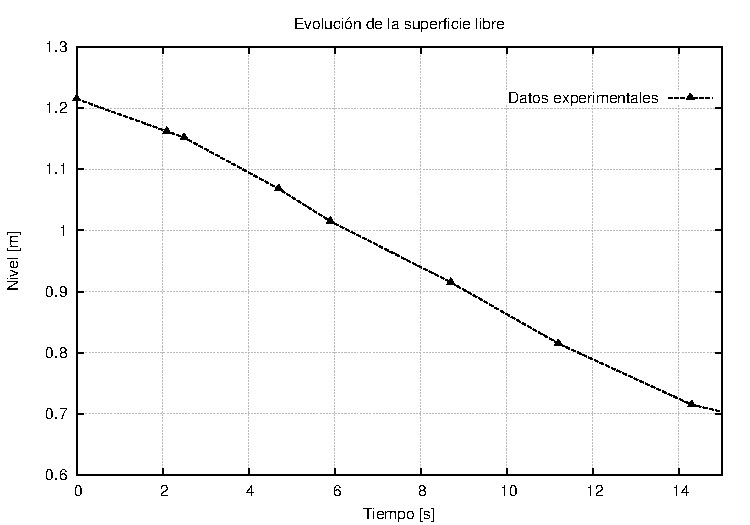
\includegraphics[scale=0.7]{hvst1.pdf}
\end{figure}
\end{frame}
\begin{frame}
{Ejemplos de aplicación}
{Análisis del segundo sistema de parada de un reactor de investigación}
Análisis de la descarga del SSP:
\begin{figure}
\centering{}
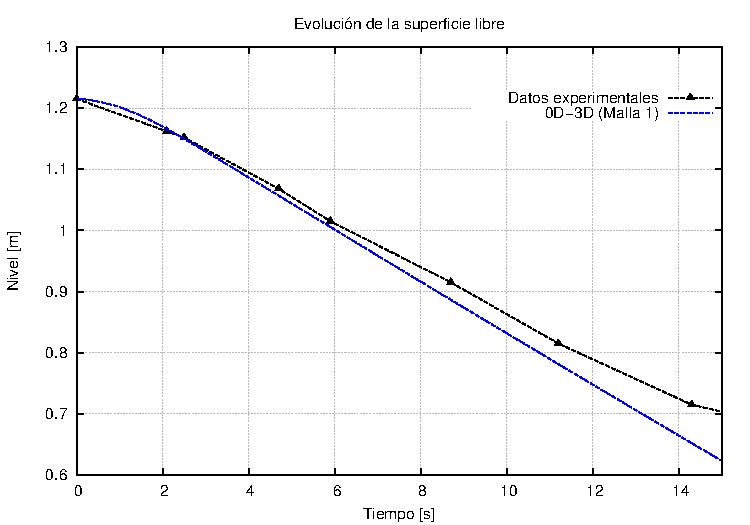
\includegraphics[scale=0.7]{hvst2.pdf}
\end{figure}
\end{frame}
\begin{frame}
{Ejemplos de aplicación}
{Análisis del segundo sistema de parada de un reactor de investigación}
Análisis de la descarga del SSP:
\begin{figure}
\centering{}
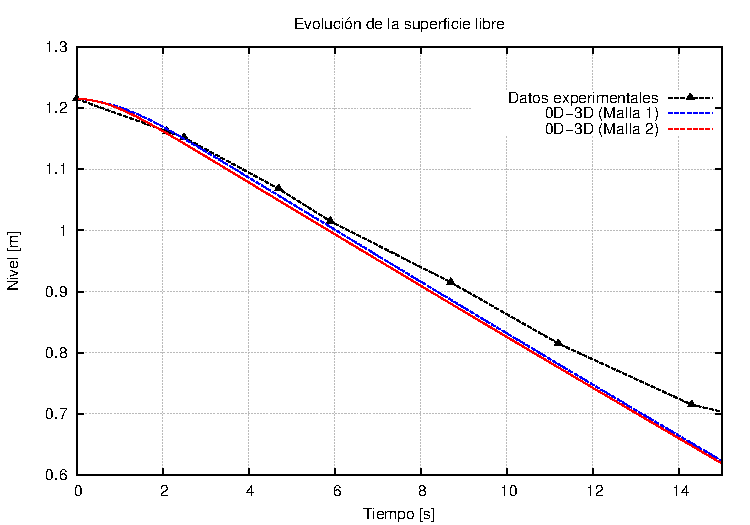
\includegraphics[scale=0.7]{hvst3.pdf}
\end{figure}
\end{frame}
\begin{frame}
{Ejemplos de aplicación}
{Análisis del segundo sistema de parada de un reactor de investigación}
Análisis de la descarga del SSP:
\begin{figure}
\centering{}
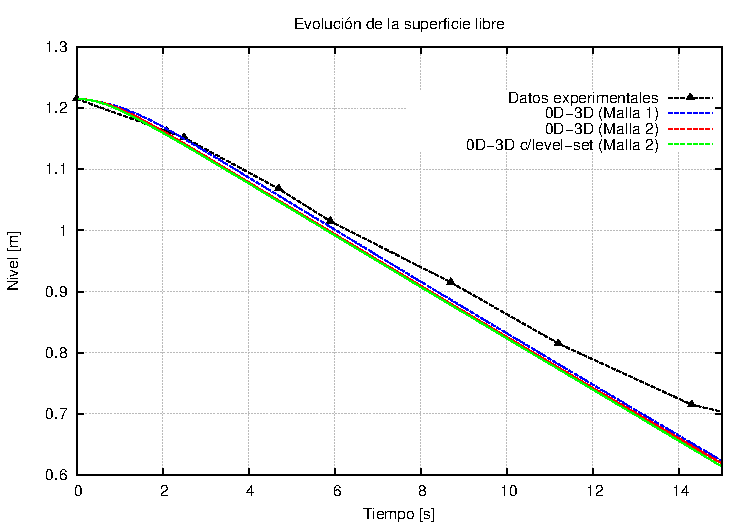
\includegraphics[scale=0.7]{hvst4.pdf}
\end{figure}
\end{frame}
\begin{frame}
{Ejemplos de aplicación}
{Análisis del segundo sistema de parada de un reactor de investigación}
Análisis de la descarga del SSP:
\begin{figure}
\centering{}
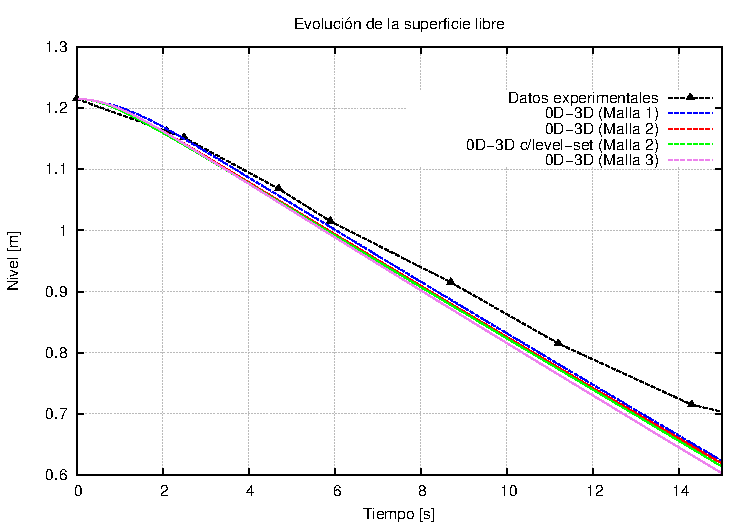
\includegraphics[scale=0.7]{hvst5.pdf}
\end{figure}
\end{frame}
\begin{frame}
{Ejemplos de aplicación}
{Análisis del segundo sistema de parada de un reactor de investigación}
Análisis de la descarga del SSP:
\begin{figure}
\centering{}
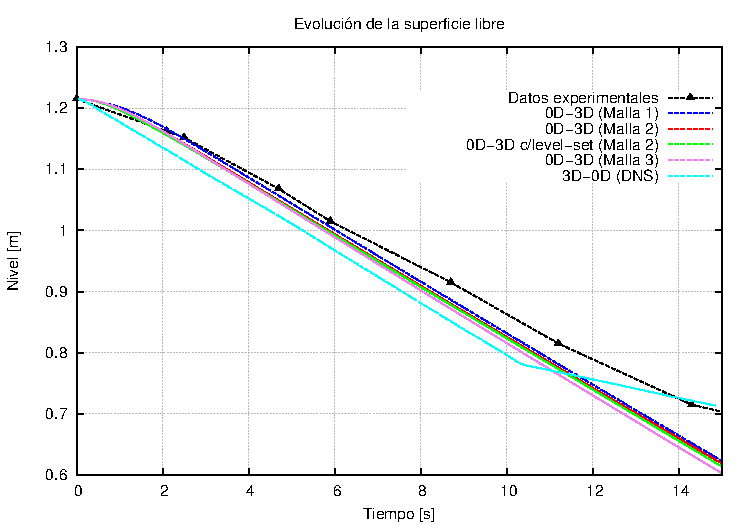
\includegraphics[scale=0.7]{hvst6.pdf}
\end{figure}
\end{frame}
\begin{frame}
{Ejemplos de aplicación}
{Análisis del segundo sistema de parada de un reactor de investigación}
Análisis de la descarga del SSP:
\begin{figure}
\centering{}
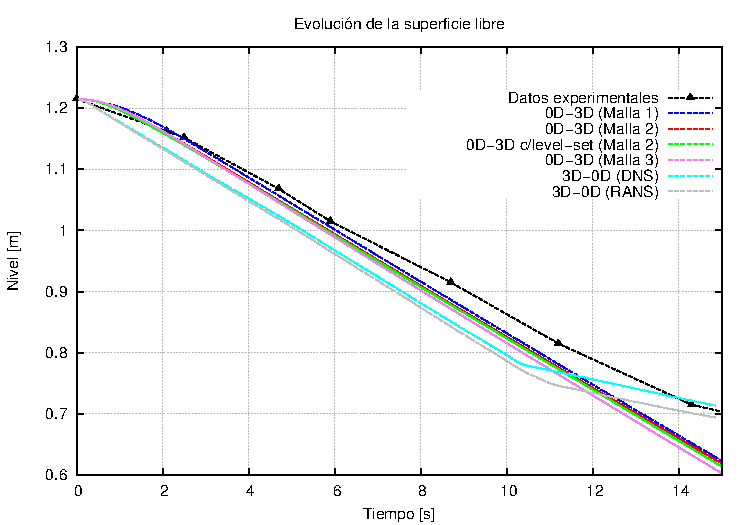
\includegraphics[scale=0.7]{hvst7.pdf}
\end{figure}
\end{frame}

\begin{frame}
{Ejemplos de aplicación}
{Análisis del segundo sistema de parada de un reactor de investigación}
Análisis de sensibilidad de resultados ante válvula en falla
\begin{figure}
\centering{}
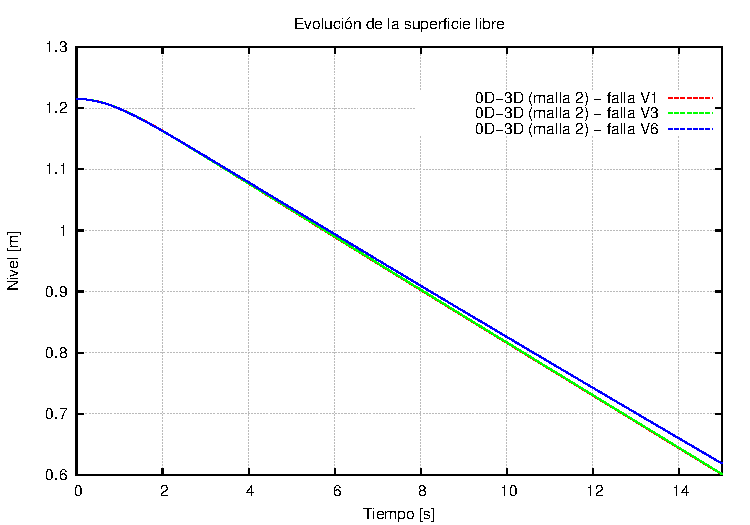
\includegraphics[scale=0.7]{hvstv.pdf}
\end{figure}
\end{frame}

\begin{frame}
{Ejemplos de aplicación}
{Análisis del segundo sistema de parada de un reactor de investigación}
Transporte de superficie libre en cañerías
\begin{equation*}
%\left\{ \begin{array}{rcl}
%\displaystyle \frac{\partial\phi}{\partial t}+ (\bar{u} \cdot \nabla) \phi &=& 0
\frac{\partial\phi}{\partial t}+ (\bar{u} \cdot \nabla) \phi = 0
\label{eq-ls}
%\end{array} \right.
\end{equation*}
\end{frame}
\begin{frame}
{Ejemplos de aplicación}
{Análisis del segundo sistema de parada de un reactor de investigación}
Transporte de superficie libre en cañerías
\begin{center}
\movie[width=1\textwidth,showcontrols=true]
{% placeholder = text or image
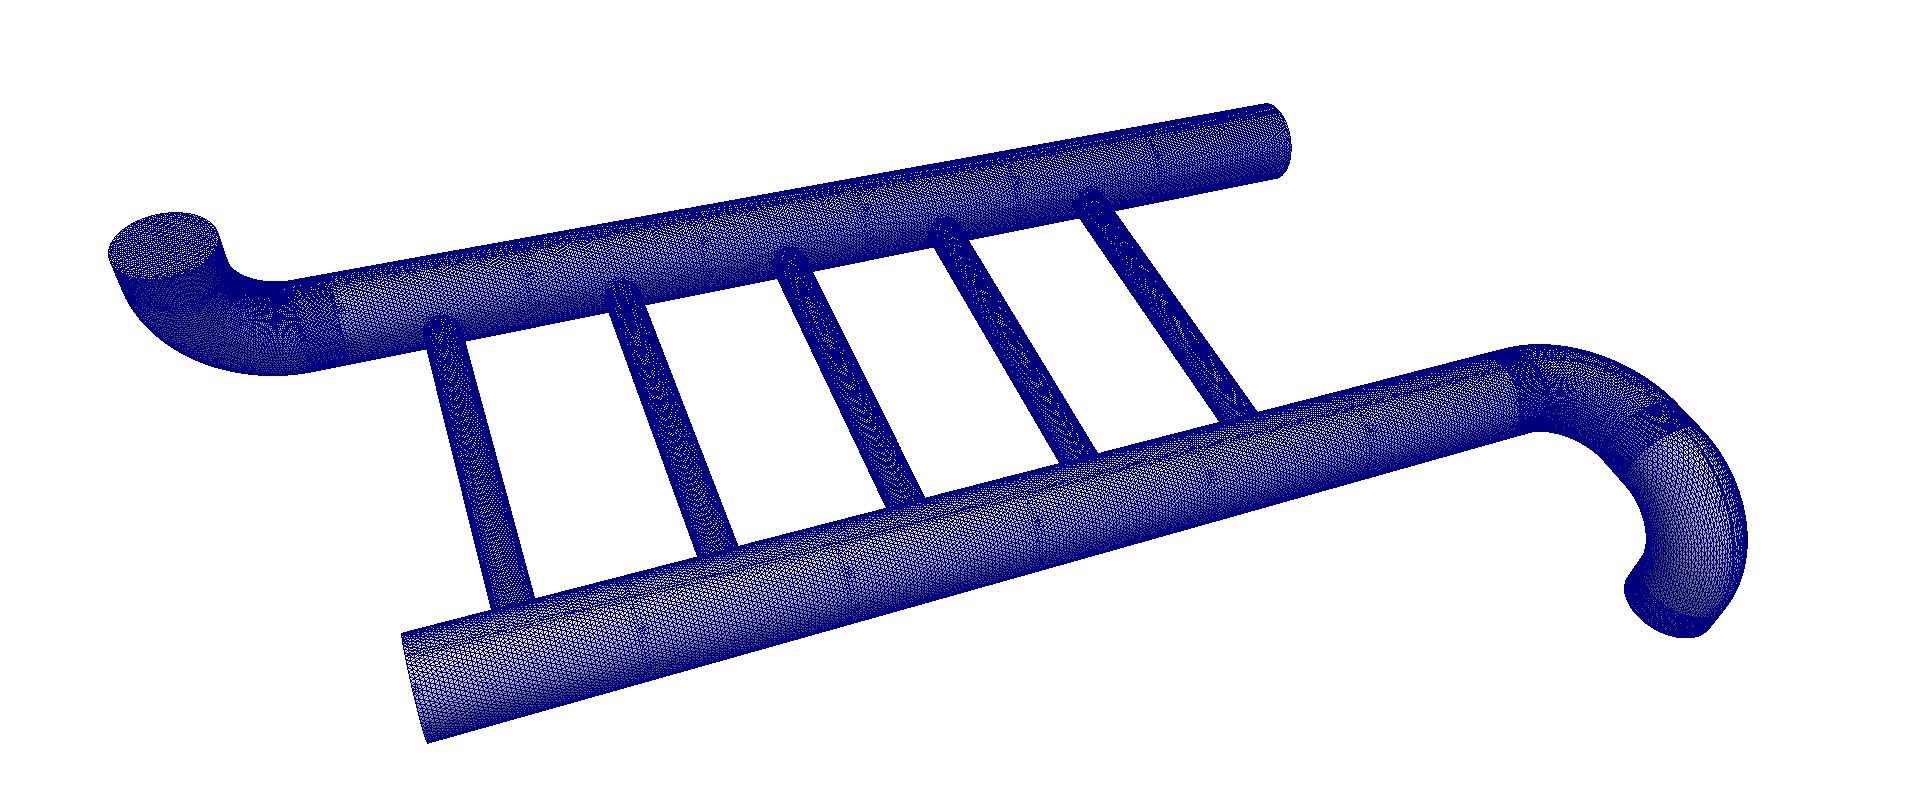
\includegraphics[width=1\textwidth]{ls-portada.png}
}%
{figs/ls.ogv} % video filename
\end{center}
\end{frame}
\begin{frame}
{Ejemplos de aplicación}
{Análisis del segundo sistema de parada de un reactor de investigación}
Transporte de superficie libre en cañerías
\begin{figure}
\centering{}
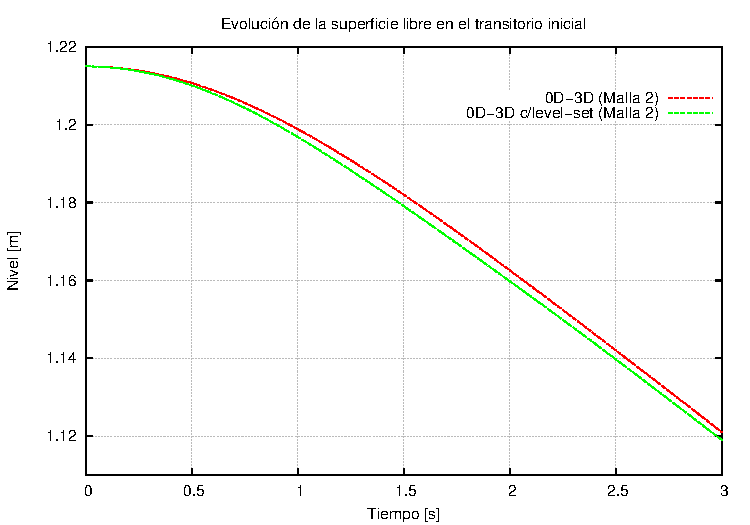
\includegraphics[scale=0.7]{hvstlsZoom.pdf}
\end{figure}
\end{frame}





\begin{frame}
{Ejemplos de aplicación}
{Análisis del segundo sistema de parada de un reactor de investigación}
Estudio de métodos numéricos para la resolución del sistema de residuos
\begin{figure}
\centering{}
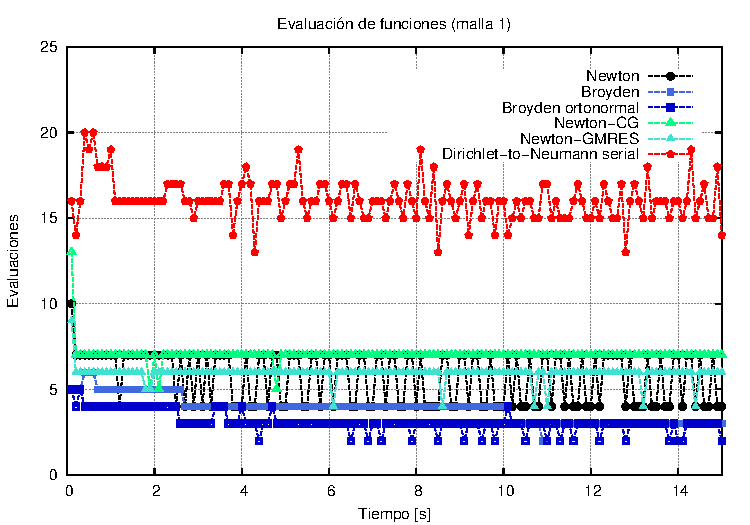
\includegraphics[scale=0.7]{nonlinear_fevals_ssp.pdf}
\end{figure}
\end{frame}







\subsection{Resolución de redes hidráulicas de múltiples componentes}

\begin{frame}
{Ejemplos de aplicación}
{Resolución de redes hidráulicas de múltiples componentes}
Descomposición disjunta de dominios en un modelo de red hidráulica con 8 incógnitas reducidas en las interfaces de acoplamiento:

\begin{figure}[ht]
\centering{}
\begin{tikzpicture}
[scale=0.8, every node/.style={scale=0.8}]

% Nodos
\node [label={\small $S_3$}] at (0em,0em) (n8) {};

\node [right of=n8, xshift=3em, yshift=-2em, align=center] (n13) {\small $v_{3}^{3}, \quad v_{5}^{1},$ \\ $P_{3}^{3}$ \quad $P_{5}^{1}$};
\node [right of=n13, xshift=3em, yshift=-2em, label={\small $S_5$}] (n14) {};
\node [right of=n14, xshift=2em, yshift=-2em] (n16) {\small $CB_{5}^{3}$};
\node [right of=n14, xshift=2em, yshift=2em] (n15) {\small $CB_{5}^{2}$};

\node [right of=n8, xshift=3em, yshift=2em, align=center] (n9) {\small $v_{3}^{2}, \quad v_{4}^{1},$ \\ $P_{3}^{2}$ \quad $P_{4}^{1}$};
\node [right of=n9, xshift=3em, yshift=0em, label={\small $S_4$}] (n10) {};
\node [right of=n10, xshift=2em, yshift=-2em] (n12) {\small $CB_{4}^{3}$};
\node [right of=n10, xshift=2em, yshift=2em] (n11) {\small $CB_{4}^{2}$};

\node [left of=n8, xshift=-3em, yshift=2em, align=center] (n7) {\small $v_{1}^{3}, \quad v_{3}^{1},$ \\ $P_{1}^{3}$ \quad $P_{3}^{1}$};
\node [left of=n7, xshift=-4em, yshift=3em, label={\small $S_1$}] (n2) {};
\node [left of=n2, xshift=-1em, yshift=-0em] (n1) {\small $CB_{1}^{1}$};

\node [right of=n2, xshift=4em, yshift=3em, align=center] (n3) {\small $v_{1}^{2}, \quad v_{2}^{1},$ \\ $P_{1}^{2}$ \quad $P_{2}^{1}$};
\node [right of=n3, xshift=3em, yshift=0em, label={\small $S_2$}] (n4) {};
\node [right of=n4, xshift=2em, yshift=2em] (n5) {\small $CB_{2}^{2}$};
\node [right of=n4, xshift=2em, yshift=-2em] (n6) {\small $CB_{2}^{3}$};

% Conexiones
\draw[|-] (n1.east) to [in=180, out=0] (n2.center);
\draw[-o] (n2.center) to[in=180, out=0] (n3.west);
\draw[-o] (n2.center) to[in=180, out=0] (n7.west);

\draw[o-] (n3.east) to[in=180, out=0] (n4.center);
\draw[-|] (n4.center) to[in=180, out=0] (n5.west);
\draw[-|] (n4.center) to[in=180, out=0] (n6.west);

\draw[o-] (n7.east) to[in=180, out=0] (n8.center);
\draw[-o] (n8.center) to[in=180, out=0] (n9.west);
\draw[-o] (n8.center) to[in=180, out=0] (n13.west);

\draw[o-] (n9.east) to[in=180, out=0] (n10.center);
\draw[-|] (n10.center) to[in=180, out=0] (n11.west);
\draw[-|] (n10.center) to[in=180, out=0] (n12.west);

\draw[o-] (n13.east) to[in=180, out=0] (n14.center);
\draw[-|] (n14.center) to[in=180, out=0] (n15.west);
\draw[-|] (n14.center) to[in=180, out=0] (n16.west);

\end{tikzpicture}
%~ \caption[Descomposición disjunta de dominios en el modelado de redes hidráulicas]
%~ {Descomposición disjunta de dominios en un modelo de red hidráulica con 16 incógnitas en las interfaces de acoplamiento.
%~ La incógnita $v_{i}^{j}$ refiere a la velocidad media en el extremo $j$ del subsistema $i$.
%~ La incógnita $P_{i}^{j}$ agrupa las presiones estática y dinámica medias en el extremo $j$ del subsistema $i$.
%~ Las incógnitas pueden reducirse rápidamente a la mitad aplicando relaciones de continuidad de campos de variables.}
%~ \label{net16}
\end{figure}

\end{frame}


\begin{frame}
{Ejemplos de aplicación}
{Resolución de redes hidráulicas de múltiples componentes}

\begin{itemize}
\item Cada subsistema se modela con ecuaciones de continuidad y de conservación de energía.
\item <2-> Ecuaciones de residuos:
\begin{equation*}
\left \{
\begin{array}{rl}
R_1 =& v_1^{2,guess} - v_1^{2,calc}(CB_1^1, P_1^{2,guess}, P_1^{3,guess}) \\
R_2 =& v_1^{3,guess} - v_1^{3,calc}(CB_1^1, P_1^{2,guess}, P_1^{3,guess}) \\
R_3 =& P_2^{1,guess} - P_2^{1,calc}(v_2^{1,guess}, CB_2^2, CB_2^3) \\
...
\end{array}
\right .
\end{equation*}
\end{itemize}
\end{frame}

\begin{frame}
{Ejemplos de aplicación}
{Resolución de redes hidráulicas de múltiples componentes}
%~ 
Redes hidráulicas con regímenes de flujo laminar:

\begin{figure}[ht]
	\begin{minipage}{0.48\linewidth}
      \centering
      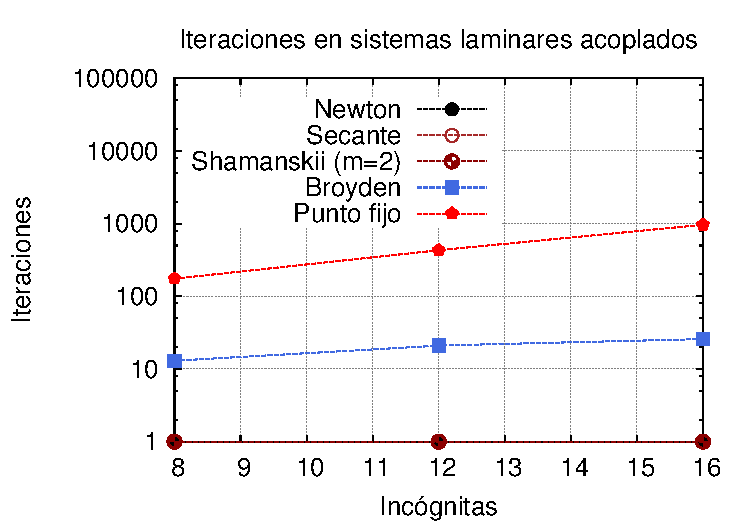
\includegraphics[scale=0.42]{net_linear_its.pdf}
		%~ \caption[]{t=0 s}
		%~ \label{asd}	
	\end{minipage}
	\begin{minipage}{0.48\linewidth}
		\centering
		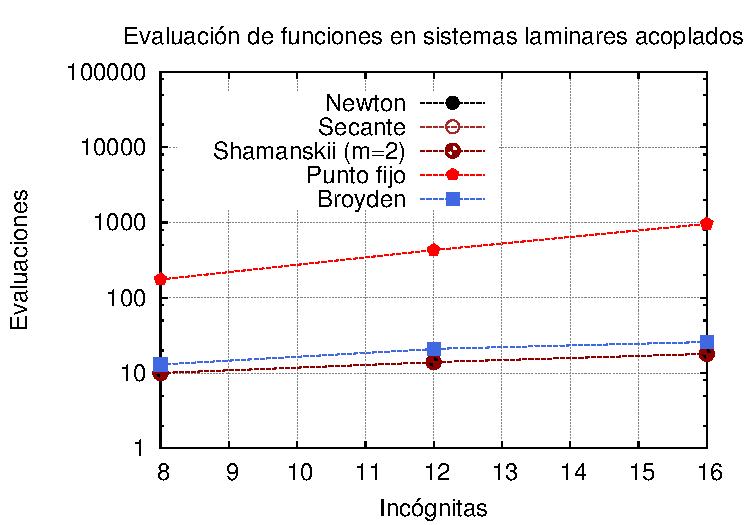
\includegraphics[scale=0.42]{net_linear_fevals.pdf}
		%~ \caption[]{t=40 s}
		%~ \label{asd}	
	\end{minipage}
\end{figure}
\end{frame}
\begin{frame}
{Ejemplos de aplicación}
{Resolución de redes hidráulicas de múltiples componentes}
Redes hidráulicas con regímenes de flujo laminar:
\begin{figure}
\centering
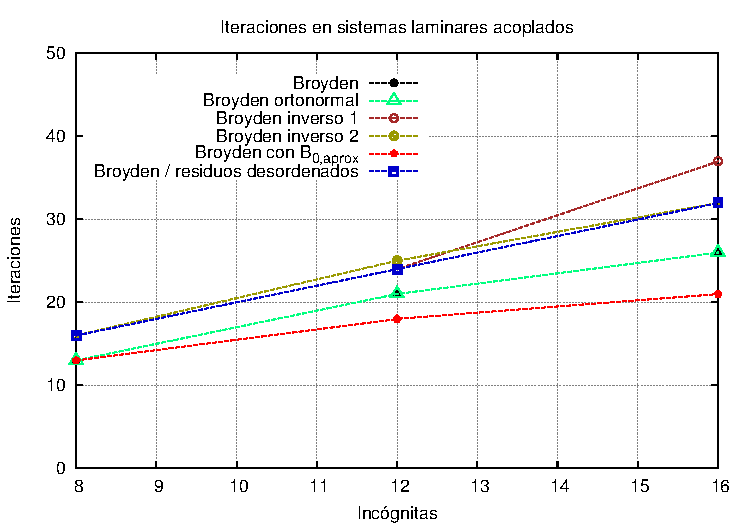
\includegraphics[scale=0.6]{net_linear_its_broy.pdf}
\end{figure}
\end{frame}

\begin{frame}
{Ejemplos de aplicación}
{Resolución de redes hidráulicas de múltiples componentes}

Redes hidráulicas con regímenes de flujo turbulento:

\begin{figure}[ht]
\centering
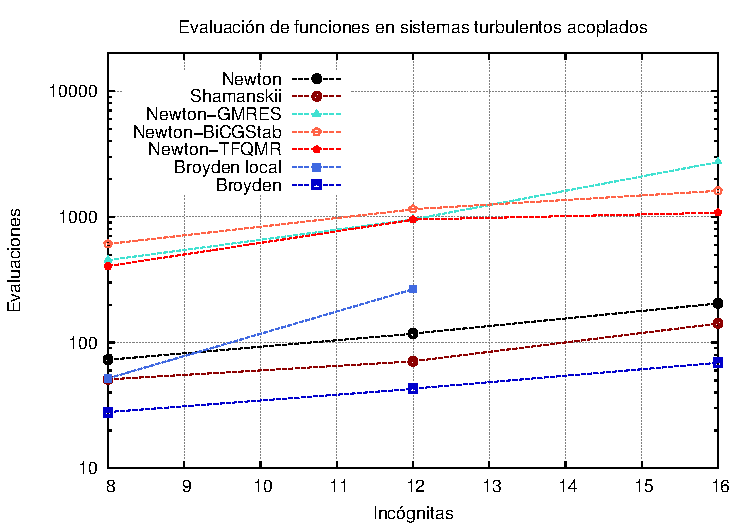
\includegraphics[scale=0.6]{net_nonLinear_fevals.pdf}
\end{figure}
\end{frame}





\subsection{Extensión a problemas acoplados en modelos de núcleo}

\begin{frame}
{Ejemplos de aplicación}
{Extensión a problemas acoplados en modelos de núcleo}

La estrategia de resolución mediante acoplamiento de códigos desarrollada puede extenderse para resolver sistemas genéricos de ecuaciones acopladas:
\begin{itemize}
  \item <2-> Las variables de acople no necesariamente deben corresponder a condiciones de borde
  \item <3-> Las variables de acople no necesariamente deben agruparse en pares
\end{itemize}
\visible<4->{
Objetivo: Modelar la dinámica del núcleo de un reactor nuclear mediante acoplamiento de códigos que resuelvan diferentes fenómenos físicos:
}
\begin{itemize}
  \item <5-> Neutrónica
    \begin{itemize}
    \item Distribución de flujo neutrónico
    \item Quemado de elementos combustibles
    \item Movimiento de barras
    \end{itemize}
  \item <6-> Termohidráulica
    \begin{itemize}
    \item Distribución de temperaturas
    \item Distribución de densidad de refrigerante
    \end{itemize}
  \item <7-> $Swelling$ de pastillas % Altera propiedades termicas (k)
  \item <8-> $Pellet-cladding$ interaction % Altera propiedades mecanicas (eps) termicas (k)
  \item <9-> Otros
\end{itemize}

\end{frame}


\begin{frame}
{Ejemplos de aplicación}
{Extensión a problemas acoplados en modelos de núcleo}
Primer modelo simplificado:
acoplamiento neutrónico-termohidráulico en cálculo de quemado de elementos combustibles.
Asumimos que:
  \begin{itemize}
    \item <2-> No hay movimiento de barras
    \item <3-> No se modela comportamiento de materiales
    \item <4-> Las secciones eficaces neutrónicas están condensadas por zonas y grupos de energía en previos cálculos de celda, y tienen dependencia con el quemado y con variables termohidráulicas
   \end{itemize}

\end{frame}


\scriptsize
\begin{frame}
{Ejemplos de aplicación}
{Extensión a problemas acoplados en modelos de núcleo}
Modelo neutrónico:

Cálculo de flujo neutrónico:
\begin{equation*}
\Delta \bar{\phi} = \frac{1}{k_{eff}}\Sigma \bar{\phi}
\label{eq-nucleo}
\end{equation*}
donde $\bar{\phi}$ es una función vectorial con el valor del flujo neutrónico en cada punto del espacio para diferentes grupos de energía,
$\Sigma$ es la matriz de secciones eficaces asociada a diferentes reacciones para diferentes grupos de energía,
y $k_{eff}$ es el factor de multiplicación del reactor.

\visible<2->{Cálculo de secciones eficaces:
\begin{equation*}
\Sigma = \Sigma \left ( N_{ref}, T_{ref}, T_{comb} \right )
\label{eq-sigma}
\end{equation*}

donde $N_{ref}$ es la densidad del refrigerante, $T_{ref}$ es la temperatura del refrigerante, $T_{comb}$ es la temperatura del combustible , 
y $B$ es el valor histórico de quemado  del material \cite{lamarsh}.
}

\visible<3->{
Cálculo de distribución de potencia:
\begin{equation*}
P = \int_{vol} E_{fis,i} \Sigma_{fis,i} \phi_{i}
\label{power}
\end{equation*}
donde $E_{fis,i}$ es la energía liberada por fisiones ocurridas en el rango de energía $i$,
$\Sigma_{fis,i}$ es la sección eficaz de fisión condensada en el grupo de energía $i$ y
$\phi_{i}$ es la componente del flujo neutrónico también condensada en el grupo de energía $i$.
}

\end{frame}



\normalsize
\begin{frame}
{Ejemplos de aplicación}
{Extensión a problemas acoplados en modelos de núcleo}

El núcleo se modela como un único canal, en contacto con una única estructura que genera energía, con diámetro del $pin$ y altura equivalente a la altura de la suma total de $pines$.

\visible<2->{La transferencia de calor a través de las estructuras de combustibles se estudia con un modelo de difusión.
}

\visible<3->{El modelo termohidráulico del refrigerante considera ecuaciones de mezcla del fluido en fases líquida y gaseosa:
\begin{itemize}
\item 2 Ecuaciones de continuidad;
\item 2 Ecuaciones de momento unidimensionales;
\item 2 Ecuaciones de conservación de energía.
\end{itemize}
}
\end{frame}

\normalsize
\begin{frame}
{Ejemplos de aplicación}
{Extensión a problemas acoplados en modelos de núcleo}

Estrategia de resolución:

\begin{itemize}
\item <2-> El código neutrónico recibe como $guess$ distribución de secciones eficaces y calcula distribución de potencia.
\item <3-> El código termohidráulico recibe como $guess$ distribución de potencias y calcula distribución de temperaturas y densidades.
\item <4-> Las variables se acoplan en zonas físicas predefinidas.
\item <5-> La evolución se discretiza en intervalos de 5 o 10 días.
\item <6-> El valor del quemado inicial es $B(\bar{x})=0$ en todo el dominio.
\item <7-> En cada intervalo temporal se actualiza el valor de $B$ por zonas físicas, considerando la distribución de potencias constante.

\end{itemize}

\end{frame}



\scriptsize
\begin{frame}
{Ejemplos de aplicación}
{Extensión a problemas acoplados en modelos de núcleo}

Acoplamiento de \textbf{Fermi} y \textbf{RELAP5} en modelo simple de núcleo:

\begin{figure}[ht]
	\begin{minipage}{0.6\linewidth}
      \centering
      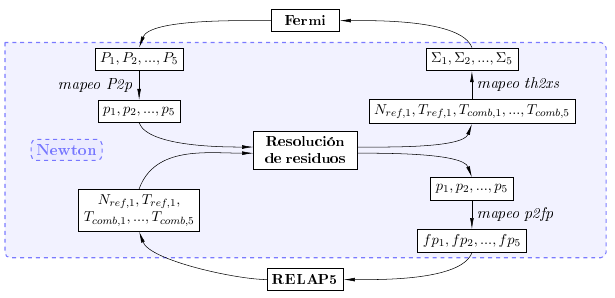
\includegraphics[scale=0.43]{esq-fermi-relap.png}
		%~ \caption[]{t=0 s}
		%~ \label{asd}	
	\end{minipage}
	\begin{minipage}{0.35\linewidth}
		\centering
		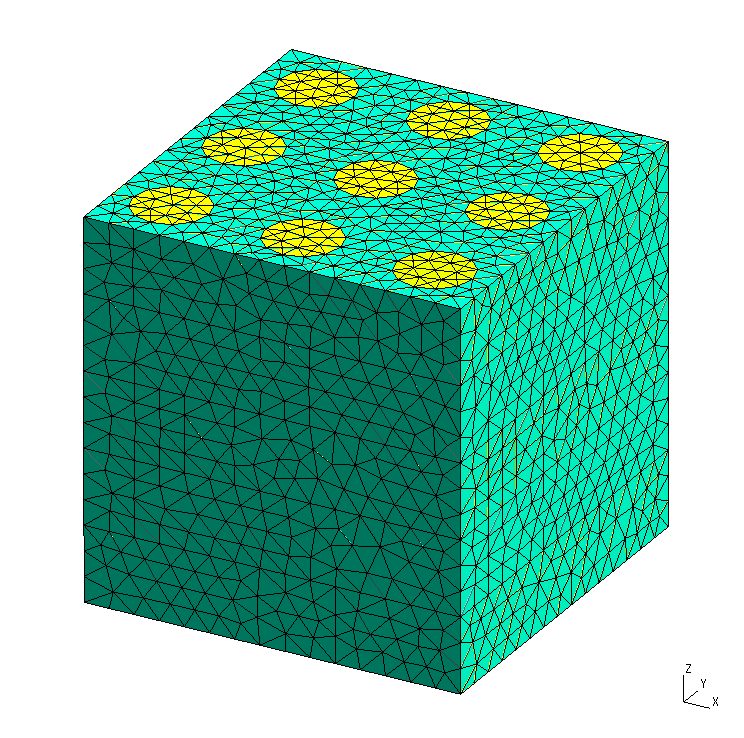
\includegraphics[scale=0.16]{fuel_z5.png}
		%~ \caption[]{t=40 s}
		%~ \label{asd}	
	\end{minipage}
\end{figure}
\visible<2->{
\begin{table}[h]
  \centering
  \begin{tabular}{c c c c cc } \hline
      \multicolumn{1}{c}{Método} & \multirow{1}{*}{$\Delta$t} & \multicolumn{1}{c}{Extrapolación} & \multicolumn{1}{c}{Extrapolación}  & \multicolumn{1}{c}{Evaluaciones} & \multicolumn{1}{c}{Tiempo} \\ % \hline
      \multicolumn{1}{c}{no lineal} & [días] & \multicolumn{1}{c}{de $\bar{x}^n$} & \multicolumn{1}{c}{de $\mathbb{J}^n$} & \multicolumn{1}{c}{totales} & \multicolumn{1}{c}{total [s]}\\ \hline %\hline
      Broyden & 10 & $\mathscr{O}(1)$ & $\mathscr{O}(1)$ & 85 & 610 \\ %\hline
      Picard & 10 & $\mathscr{O}(1)$ & - & 68 & 684 \\ %\hline
      Punto fijo & 10 & $\mathscr{O}(1)$ & - & 87 & 628  \\ %\hline
      Shamanskii & 10 & $\mathscr{O}(1)$ & $\mathscr{O}(0)$& 370 & 2663  \\ \hline
   \end{tabular}   
   \caption[Evaluaciones totales y tiempo total requerido por cada método no lineal en cálculo de quemado con \textbf{RELAP5} y \textbf{Fermi}]
   {\scriptsize Evaluaciones totales y tiempo total requerido por cada método no lineal.}
   \label{tabla-relap-fermi}
\end{table}
}

\end{frame}




\normalsize
\begin{frame}
{Ejemplos de aplicación}
{Extensión a problemas acoplados en modelos de núcleo}

Acoplamiento de \textbf{PUMA} y \textbf{RELAP5} en modelo de núcleo de CAREM-25:

\begin{figure}[ht]
	\begin{minipage}{0.48\linewidth}
      \centering
      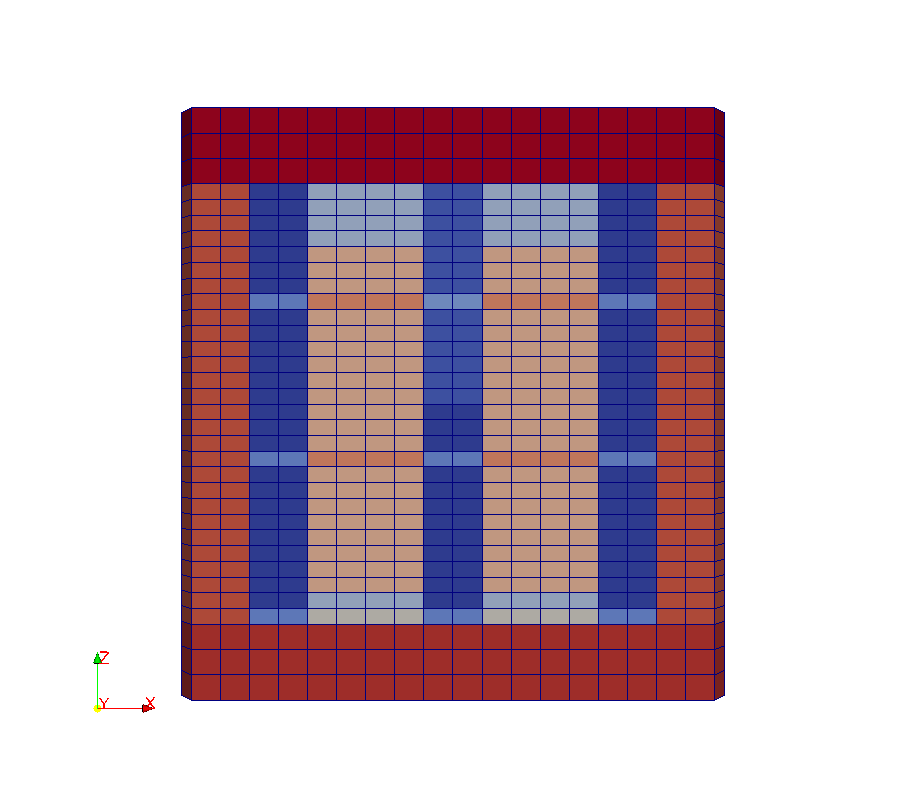
\includegraphics[scale=0.18]{carem_geom_1.png}
		%~ \caption[]{t=0 s}
		%~ \label{asd}	
	\end{minipage}
	\begin{minipage}{0.48\linewidth}
		\centering
		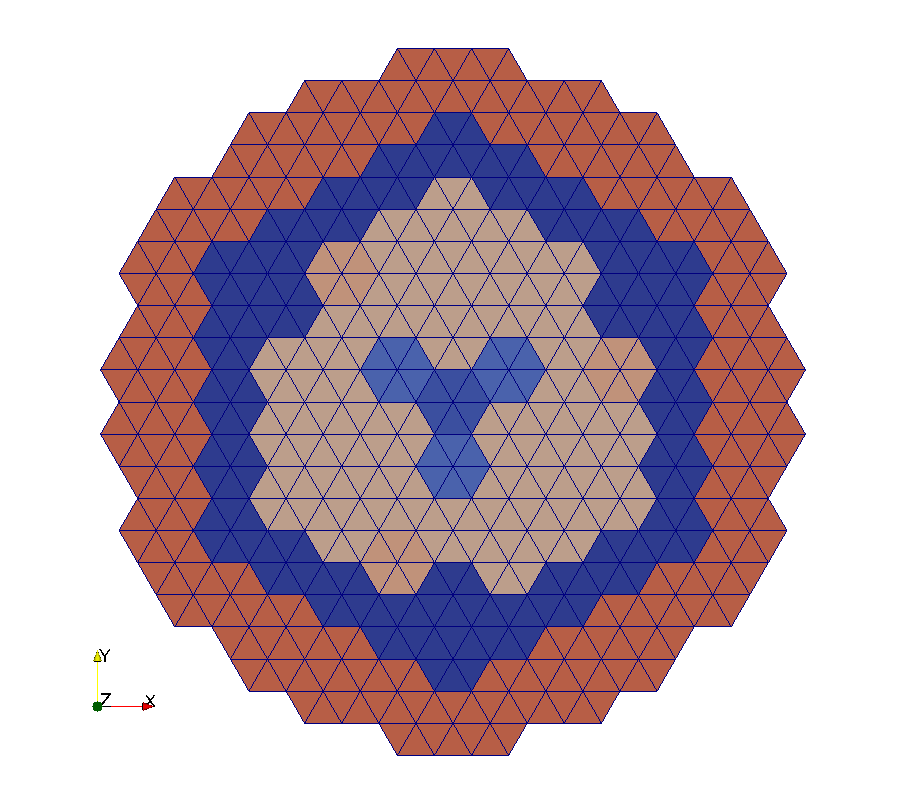
\includegraphics[scale=0.15]{carem_geom_2.png}
		%~ \caption[]{t=40 s}
		%~ \label{asd}	
	\end{minipage}
\end{figure}

\end{frame}



\scriptsize
\begin{frame}
{Ejemplos de aplicación}
{Extensión a problemas acoplados en modelos de núcleo}

Acoplamiento de \textbf{PUMA} y \textbf{RELAP5} en modelo de núcleo de CAREM-25:

\begin{figure}[ht]
	\begin{minipage}{0.48\linewidth}
      \centering
      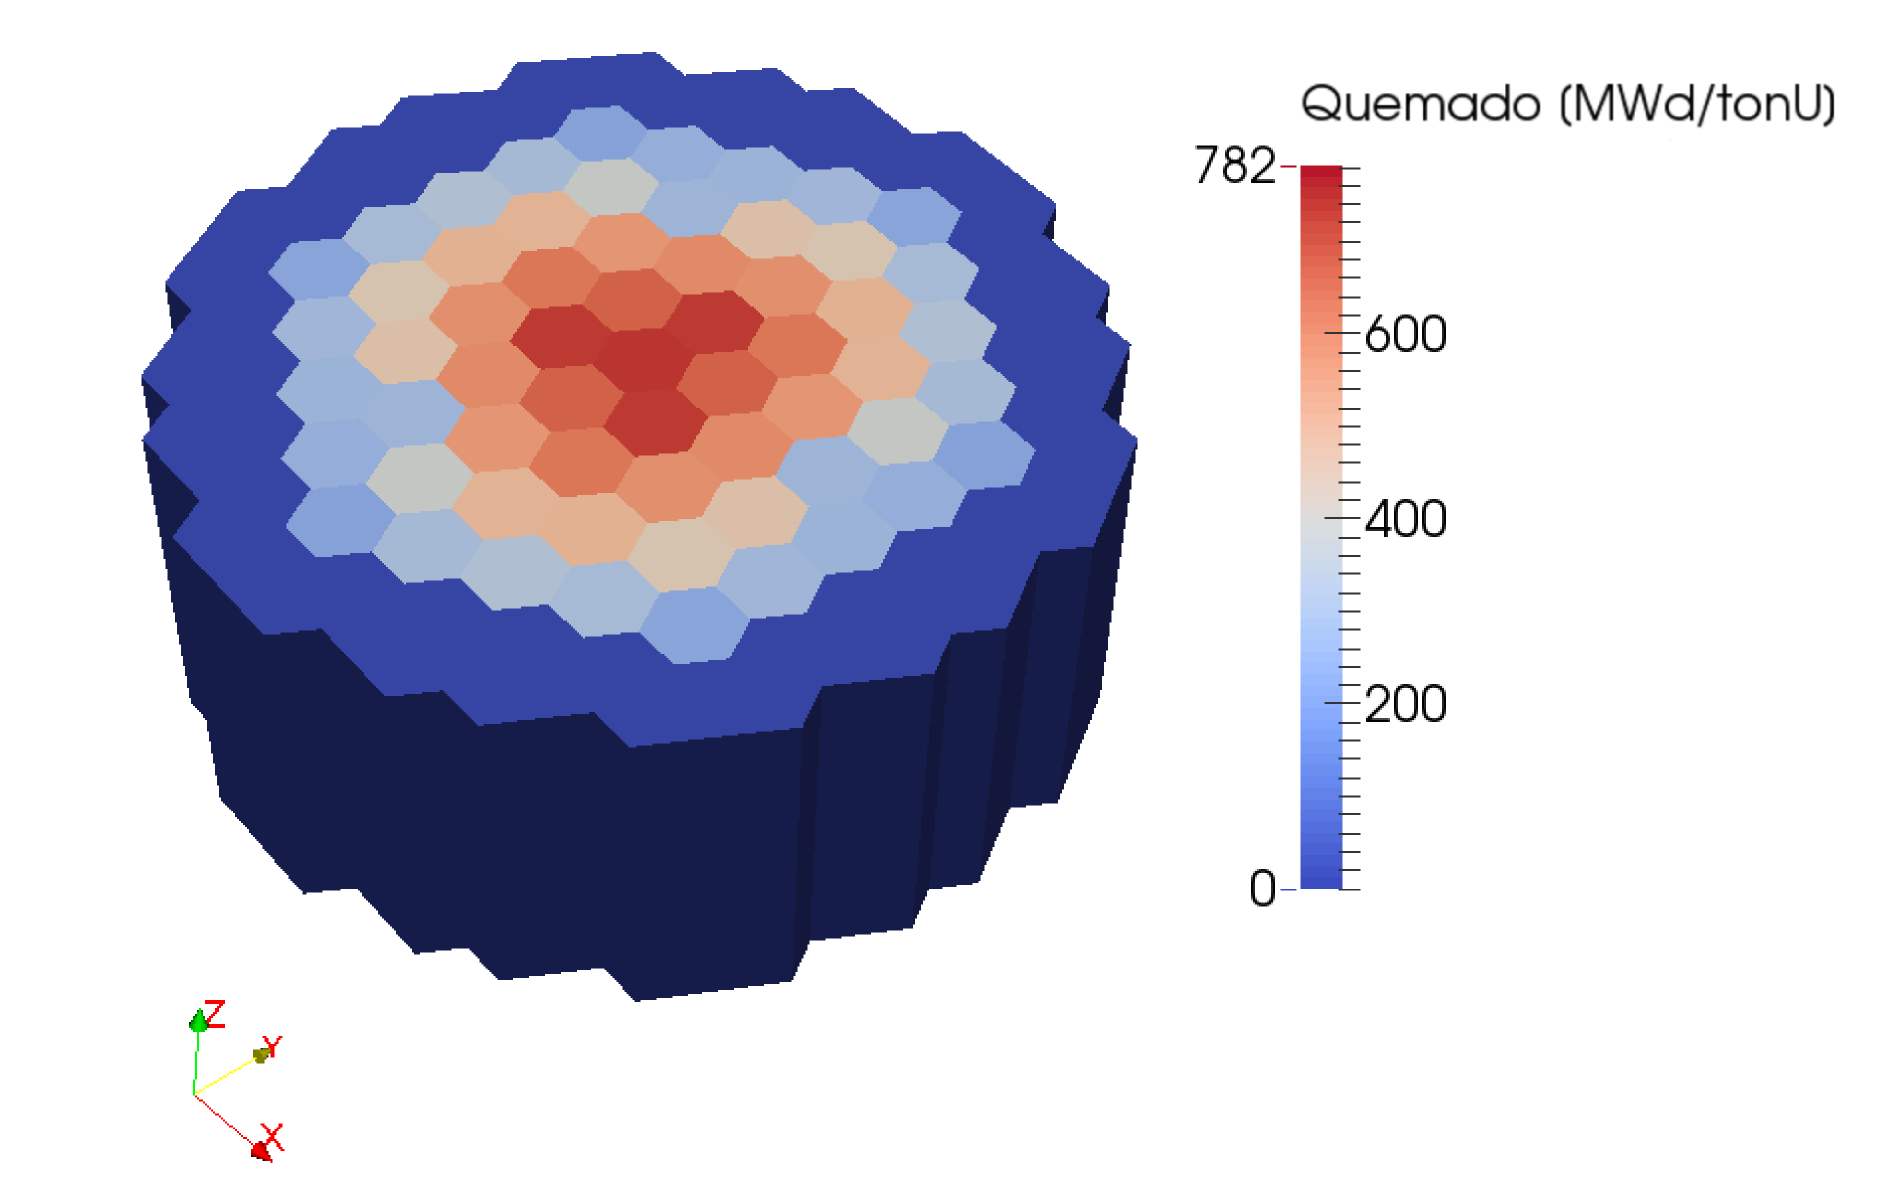
\includegraphics[scale=0.06]{carem_burnup_10day.png}
		\caption[]{t=10 días}
		%~ \label{asd}	
	\end{minipage}
	\begin{minipage}{0.48\linewidth}
		\centering
		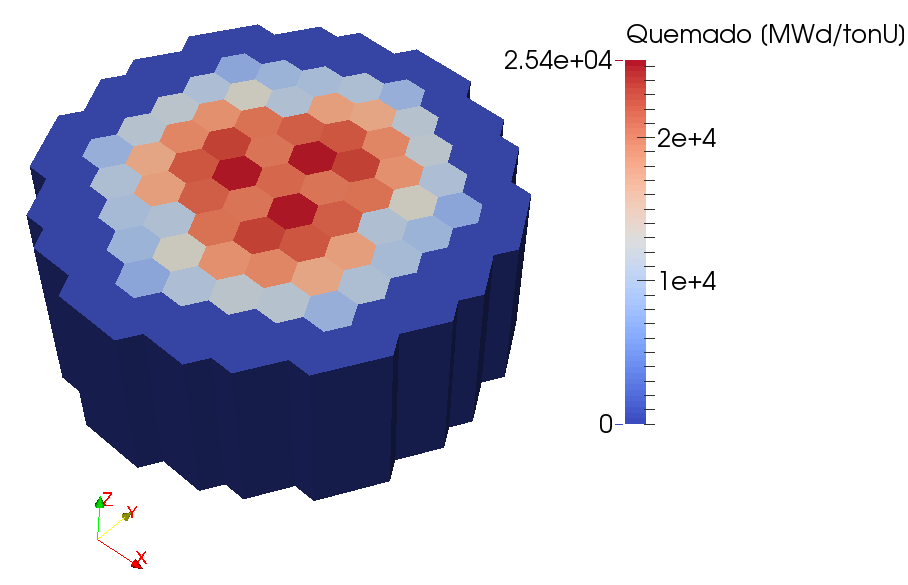
\includegraphics[scale=0.12]{carem_burnup_400day.png}
		\caption[]{t=400 días}
		%~ \label{asd}	
	\end{minipage}
\end{figure}
\visible<2->{

\begin{table}[h!]
  \centering
  \begin{tabular}{ c c c c c } 
      \hline
      \multicolumn{1}{c}{Método} & \multirow{1}{*}{$\Delta$t} & \multicolumn{1}{c}{Extrapolación} & \multicolumn{1}{c}{Evaluaciones} & \multicolumn{1}{c}{Tiempo} \\ % \hline
      \multicolumn{1}{c}{no lineal} & [días] & \multicolumn{1}{c}{de $\bar{x}^n$} & \multicolumn{1}{c}{totales} & \multicolumn{1}{c}{total [s]}\\ \hline %\hline
      Picard & 5 & $\mathscr{O}(0)$ & 243 & 11019 \\ %\hline
      Picard & 5 & $\mathscr{O}(1)$ & 195 & 9085  \\ %\hline
      Picard & 10 & $\mathscr{O}(0)$ & 131 & 5898 \\ %\hline            
      Picard & 10 & $\mathscr{O}(1)$ & 104 & 4774 \\ %\hline            
      Punto fijo & 5 & $\mathscr{O}(0)$ & 139 & 5415 \\ %\hline            
      Punto fijo & 5 & $\mathscr{O}(1)$ & 186 & 6990 \\ %\hline            
      Punto fijo & 10 & $\mathscr{O}(0)$ & 101 & 3755  \\ % \hline      
      Punto fijo & 10 & $\mathscr{O}(1)$ & 107 & 3919  \\ \hline            
   \end{tabular}   
   \caption[Evaluaciones totales y tiempo total requerido por cada método no lineal en cálculo de quemado con \textbf{RELAP5} y \textbf{Fermi}]
   {\scriptsize Evaluaciones totales y tiempo total requerido por cada método no lineal.}
   \label{tab-relap-puma}
\end{table}



}

\end{frame}
